\documentclass[12pt]{extarticle}
\usepackage{tempora}
\usepackage[T1, T2A]{fontenc}
\usepackage[utf8]{inputenc}
\usepackage[english, ukrainian]{babel}
\usepackage{geometry}
\usepackage{graphicx}
\usepackage{multirow}
\usepackage{multicol}
\usepackage{float}
\graphicspath{{/home/artem/Pictures}}
\geometry
{
    a4paper,
    left=30mm,
    top=15mm,
    right=20mm,
    bottom=15mm,
}

\begin{document}
\begin{titlepage}
    \begin{center}
        \textbf{\normalsize{\MakeUppercase{
            Міністерство Освіти і науки України
            Національний університет "Львівська політехніка"
        }}}

        \begin{flushright}
        \textbf{ІКНІ}\\
        Кафедра \textbf{ПЗ}
        \end{flushright}
        \vspace{15mm}

        \includegraphics[width=0.4\textwidth]{lpnu_logo.png}

        \vspace*{\fill}

        \textbf{\normalsize{\MakeUppercase{Звіт}}}
            
        До лабораторної роботи №3

        \textbf{на тему:} “Створення та керування процесами засобами API в операційній
        системі WINDOWS”

        \textbf{з дисципліни:} “Операційні системи”
            
        \vspace*{\fill}

        \begin{flushright}

            \textbf{Лектор:}\\
            старший викладач кафедри ПЗ\\
            Грицай О.Д.\\
            \vspace{12pt}

            \textbf{Виконав:}\\
            студент групи ПЗ-24\\
            Губик А. С.\\
            \vspace{12pt}

            \textbf{Прийняв:}\\
            доцент кафедри ПЗ\\
            Горечко О. М.\\
        \vspace{12pt}
        \end{flushright}

        Львів -- 2023
            
            
    \end{center}
\end{titlepage}

\textbf{Тема роботи:}Створення та керування процесами засобами API в операційній
системі WINDOWS
\vspace{12pt}

\textbf{Мета роботи:} Ознайомитися з багатопоточністю в ОС Windows. Навчитися
працювати з процесами, використовуючи WinAPI-функції.

\subsection*{Теоретичні відомості}
Ядро операційної системи є основною частиною, що забезпечує
інтерфейс між прикладними програмами та апаратним забезпеченням
комп’ютера. Фактично, це програма, процеси якої постійно виконуються.
Функції ядра забезпечують фундаментальні механізми (такі, як
планування потоків, синхронізація), які використовуються компонентами
виконавчої системи та низькорівневими апаратно-залежними засобами
підтримки (диспетчеризації переривань і винятків).
Функції ядра відокремленні від функцій решти виконавчої системи.
Ядро відповідає за системні механізми і не бере участі в управлінні
завданнями, що пов'язані зі системною політикою. До завдань виконавчої
системи належать практично всі, крім планування і диспетчеризації
потоків.
За межами ядра виконавча система представляє потоки та інші
поділювані ресурси у вигляді об'єктів. Управління цими об'єктами
вимагає певних витрат, так як потрібні дескриптори, що дозволяють
маніпулювати об'єктами, засоби захисту та квоти ресурсів, що
резервуються при їх створенні. Ядро реалізує набір більш простих
об'єктів, що називаються об'єктами ядра (kernel objects). Ці об'єкти
дозволяють ядру контролювати обробку даних процесором і підтримують
об'єкти виконавчої системи. Більшість об'єктів рівня виконавчої системи
інкапсулюють один або більше об'єктів ядра, включаючи в себе їх
атрибути, визначені ядром. Об'єкти ядра використовуються системою і
прикладними додатками для управління безліччю різних ресурсів:
процесами, потоками, файлами і т.д.
Система дозволяє створювати і оперувати декількома типами таких
об'єктів, в тому числі: маркерами доступу (access token objects), файлами
(file objects), відображеннями (проекціями) файлів (file-mapping objects),
портами завершення введення виведення (I / O completion port objects),
завданнями (jobs), поштовими скриньками (mailslot objects), м'ютексами
(mutex objects), каналами (pipe objects), процесами (thread objects) і
таймерами очікування (waitable timer objects). Ці об'єкти створюються
Windows-функціями. Наприклад, CreateFileMapping змушує систему
створити об'єкт відображення файлу.

\subsection*{Хід роботи}


\paragraph{I.}.
\begin{figure}[H]
    \centering
    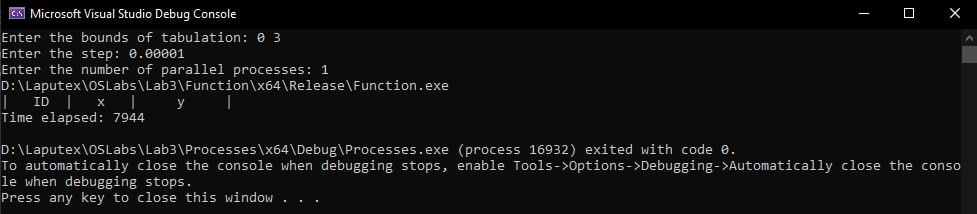
\includegraphics[width=0.90\textwidth]{func.jpg}
    \caption{top}
\end{figure}

\begin{center}
    \begin{tabular}{| c | c | c | c |}
        \hline
        Діапозон &Крок& К-сть процесів & Час виконання(ms)\\
        \hline
        0 - 3 &  0.1  & 1 & 78 \\
        0 - 3 &  0.1  & 4 & 148 \\
        \hline
        0 - 3 &  0.0001  & 1 & 6021 \\
        0 - 3 &  0.0001  & 2 & 8749 \\
        \hline
        0 - 3 &  0.000001  & 1 & 97681 \\
        0 - 3 &  0.000001  & 12 & 33821 \\
        \hline
   
    \end{tabular}

\end{center}
\paragraph{II.}.

\begin{figure}[H]
    \centering
    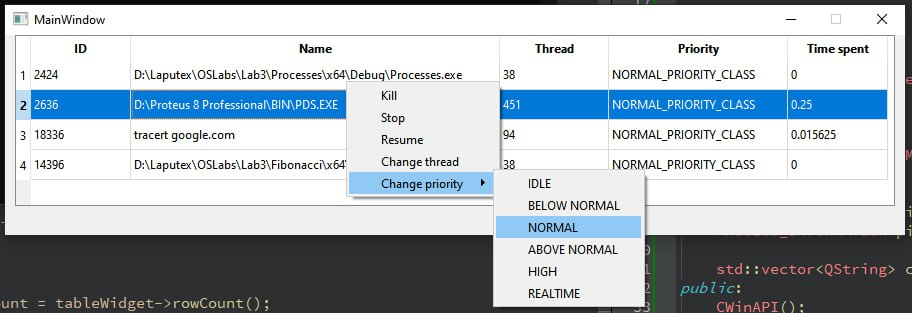
\includegraphics[width=0.90\textwidth]{ui.jpg}
    \caption{qps}
\end{figure}
\begin{figure}[H]
    \centering
    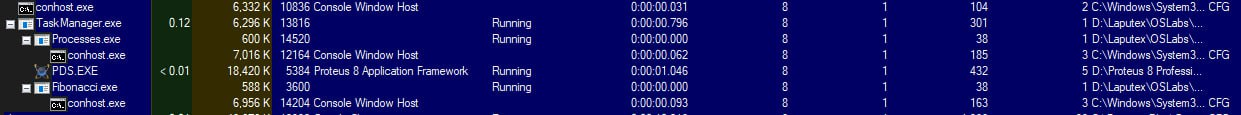
\includegraphics[width=0.90\textwidth]{exp.jpg}
    \caption{top}
\end{figure}
\textbf{Висновок:}
Я навчився створювати процеси і отримувати про них інформацію.
 \end{document}
